% TO DO: add citations in thesis work, better research plan

\documentclass[10pt]{beamer}
\usetheme[height=0mm]{Rochester}
\usecolortheme{}
\usefonttheme[onlylarge]{structurebold}
\setbeamerfont*{frametitle}{size=\normalsize,series=\bfseries}
\setbeamertemplate{navigation symbols}{}
\setbeamercovered{dynamic}
\setbeamertemplate{itemize item}[triangle]
\setbeamertemplate{itemize subitem}[triangle]

%  use Darmstadt if commenting the next line
\usepackage[footheight=1em]{beamerthemeboxes}
\usepackage[natbib=true,backend=biber,citestyle=authoryear]{biblatex}
\bibliography{../bib/stats,../bib/learning}

\usepackage{amsmath,amssymb,amsthm,bbm}             % AMS Math
\usepackage[utf8]{inputenc}
\usepackage[english]{babel}
\usepackage{xcolor}
\usepackage{graphicx}
\usepackage{subfigure}
\usepackage{hyperref}
\usepackage{mathtools}
\usepackage{mathrsfs}
% notation
\DeclareMathOperator*{\argmax}{arg\,max}
\DeclareMathOperator*{\argmin}{arg\,min}
\newcommand{\cA}{\mathcal{A}}
\newcommand{\cS}{\mathcal{S}}
\newcommand{\cF}{\mathcal{F}}
\newcommand{\cX}{\mathcal{X}}
\newcommand{\cY}{\mathcal{Y}}
\newcommand{\cZ}{\mathcal{Z}}
\newcommand{\cN}{\mathcal{N}}
\newcommand{\cO}{\mathcal{O}}
\renewcommand{\leq}{\leqslant}
\renewcommand{\geq}{\geqslant}
\renewcommand{\phi}{\varphi}
\renewcommand{\epsilon}{\varepsilon}
\renewcommand{\d}{ {\rm d}}
\renewcommand{\emptyset}{\varnothing}

\usepackage{tikz}
\usetikzlibrary{bayesnet}
\usetikzlibrary{arrows}
\usepackage{url}

\definecolor{bleu}{rgb}{0.2,0.4,0.65}
\setbeamercolor{palette primary}{bg=bleu,fg=white}
\setbeamercolor{palette secondary}{bg=bleu,fg=white}
\setbeamercolor{palette tertiary}{bg=bleu,fg=white}
\setbeamercolor{palette quaternary}{bg=bleu,fg=white}
\setbeamercolor{structure}{fg=bleu} % itemize, enumerate, etc
\setbeamercolor{section in toc}{fg=bleu} % TOC sections
\def\figdir{Figures}

\setbeamertemplate{footline}[frame number]

\AtBeginSection[] % Do nothing for \section*
{
\begin{frame}
\frametitle{Outline}
\tableofcontents[currentsection]
\end{frame}
}

\newcommand{\backupbegin}{
   \newcounter{framenumberappendix}
   \setcounter{framenumberappendix}{\value{framenumber}}
}
\newcommand{\backupend}{
   \addtocounter{framenumberappendix}{-\value{framenumber}}
   \addtocounter{framenumber}{\value{framenumberappendix}}
}
\makeatletter


\title[Bayesian ML: Bayesics]{BML lecture \#1: Bayesics}
\subtitle{\url{http://github.com/rbardenet/bml-course}}
\author[Rémi Bardenet (CNRS \& Univ. Lille)] % (optional, for multiple authors)
{Rémi Bardenet\\ \url{remi.bardenet@gmail.com}}
\institute[] % (optional)
{
  CNRS \& CRIStAL, Univ. Lille, France\\
\vspace{1cm}
\includegraphics[width=0.15\textwidth]{/Users/rbardenet/Work/Tex/PosterImages/logoCNRS.pdf}
\qquad \includegraphics[width=0.4\textwidth]{/Users/rbardenet/Work/Tex/PosterImages/cristalLogo.pdf}
}
\date{}

\begin{document}
\begin{frame}
\maketitle
\end{frame}

\begin{frame}{What comes to $your$ mind when you hear "Bayesian ML"?}

\end{frame}

\begin{frame}{Course outline}

\end{frame}

\begin{frame}
\frametitle{Outline}
\tableofcontents
\end{frame}

%%%%%%%%%%%%%%%%%%%%%%
% \section{Introduction}
% %%%%%%%%%%%%%%%%%%%%%%

% \begin{frame}
%   \frametitle{A quick motivating example before we go formal 1/2}
%   \begin{itemize}
%     \vfill\item Let $N$ individuals evolve from Susceptible to Infected to Recovered, $x_n(t) \in\{S,I,R\}$, $1\leq n\leq N$, $t\in[0,T]$.
%     \vfill\item Each susceptible individual $n$ moves to $I$ according to a Poisson process with intensity
%     $$\sum_{k:x_k(t)=I} \lambda_{nk}(\unn{\theta_{SI}}).$$
%     \vfill\item Each infected person recovers after a Gamma(\unn{$a,b$}) time.
%     \vfill\item This allows to express
%     $$
%     p(x_1(t_{1,1}), \dots, x_1(t_{1,T_1}), \cdots, x_N(t_{N,1}), \dots, x_1(t_{N,T_N})\vert \unn{\theta}).
%     $$
%     where \unn{$\theta= (\theta_{SI}, a, b)$}.
%     \vfill\item Now, consider $p(\theta\vert \text{data}) \propto p(\text{data}\vert \theta) \un{p(\theta)}.$
%   \end{itemize}
% \end{frame}

% \begin{frame}
% \frametitle{A quick motivating example before we go formal 2/2}
%   \begin{itemize}
%   \vfill\item If asked to report an interval $A$ on a particular function of $\theta$, say $R_0 = h(\theta)$, I would report a small interval $A$ such that
%   $$ \int 1_{h(\theta)\in A} \, p(\theta\vert \text{data}) \,\d\theta = p (h(\theta)\in A \vert \text{data}) \geq 0.95.$$
%   \vfill\item If asked whether we should close universities, I would ask for
%   \begin{itemize}
%     \item \un{the cost $\alpha$ of closing unis when $R_0<1$},
%     \item \unn{the cost $\beta$ of keeping unis open while $R_0>1$}.
%   \end{itemize}
%   \vfill\item Then I would recommend closing if and only if
%   $$
%   p(R_0>1\vert \text{data}) > \frac{\un{\alpha}}{\un{\alpha}+\unn{\beta}}.
%   $$
%   \vfill\item Additionally, I would check that the decision doesn't change if I change my prior $p(\theta)$ a little.
%   \vfill\item If it did, then I would refine my likelihood and/or wait for more data.
% \end{itemize}
%   % \tikz{ %
%   %   \node[latent] (S) {$S$};%
%   %   \node[latent,right=of S] (I) {$I$}; %
%   %   \node[latent,right=of I] (R) {$R$}; %
%   %   \edge S I;
%   %   \edge I R;
%   % }
% \end{frame}

\begin{frame}{Quotes from \cite{GCSDVR13} on Bayesian methods}
% put book picture
\begin{itemize}
 \vfill\item \emph{[...] practical methods for making inferences from data, using probability models for quantities we observe \un{and for quantities about which we wish to learn}.}
\vfill\item \emph{The essential characteristic of Bayesian methods is their \un{explicit use of probability for quantifying uncertainty} in inferences based on statistical data analysis.}
\vfill\item \emph{Three steps:
\begin{enumerate}
  \item Setting up a full probability model,
  \item Conditioning on observed data, calculating and interpreting the appropriate ``posterior distribution",
  \item Evaluating the fit of the model and the implications of the resulting posterior distribution. In response, one can alter or expand the model and repeat the three steps.
\end{enumerate}
}
\end{itemize}
\end{frame}

\begin{frame}{Notation that I will try to stick to}
\begin{itemize}
  \vfill\item $y_{1:n} = (y_1,\dots,y_n) \in \cY^n$ denote observable data/labels.
  \vfill\item $x_{1:n} \in \cX^n$ denote covariates/features/hidden states.
  \vfill\item $z_{1:n} \in \cZ^n$ denote hidden variables.
  \vfill\item $\theta\in\Theta$ denote parameters.
  \vfill\item $X$ denotes an $\cX$-valued random variable. Lowercase $x$ denotes either a point in $\cX$ or an $\cX$-valued random variable.
\end{itemize}
\end{frame}

\begin{frame}{More notation}
  \begin{itemize}
  \vfill\item Whenever it can easily be made formal,
  %(by choosing an appropriate reference $\sigma$-finite measure, say Lebesgue or the counting measure),
  we write densities for our random variables and let the context indicate what is meant. So if $X\sim \cN(0,\sigma^2)$, we write
  $$ \mathbb E h(X) = \int h(x) \frac{e^{-x^2/2\sigma^2}}{\sigma\sqrt{2\pi}}\d x = \int h(x)p(x)\mathrm{d}x.$$
  Similarly, for $X\sim \mathcal P(\lambda)$, we write
  $$ \mathbb E h(X) = \sum_{k=0}^\infty h(k) e^{-\lambda}\frac{\lambda^k}{k!} = \int h(x) p(x)\mathrm{d} x$$
  \vfill\item All pdfs are denoted by $p$, so that, e. g.
  \begin{align*}
\mathbb{E} h(Y, \theta) &= \int h(y, \theta)p(y, \theta)\,\d y\d \theta\\
&= \int h(y, \theta)p(y, x, \theta) \,\d x\d y \d\theta\\
&= \int h(y, \theta) p(y, \theta\vert x)p(x) \,\d x\d y \d\theta
  \end{align*}
\end{itemize}
\end{frame}

% \begin{frame}{Make sure you're in the right class}
%   \begin{center}
%     \includegraphics[width=\onefig]{Figures/bodybuilding}
%   \end{center}
%   \end{frame}
   
%   \begin{frame}
%     \frametitle{These are more the applications we have in mind}
%     \only<1>{
%     \fbox{
%       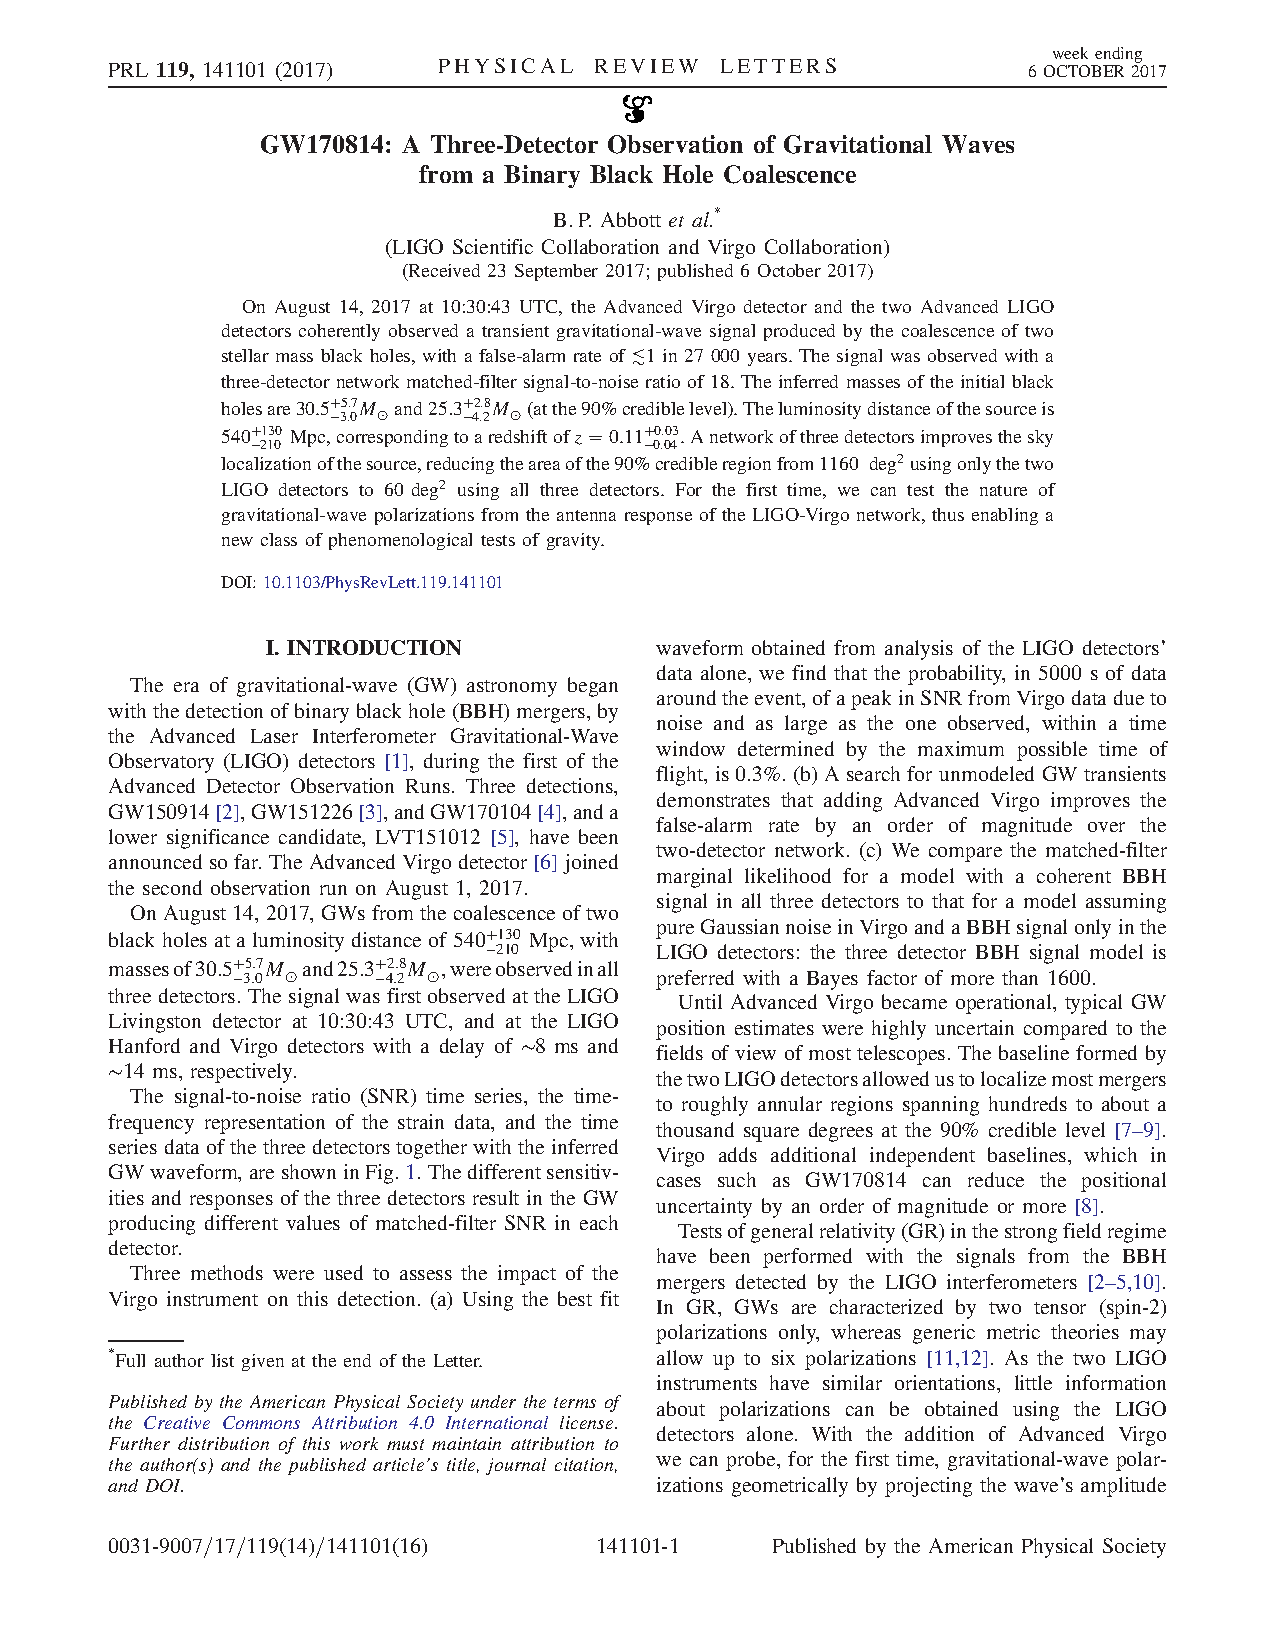
\includegraphics[trim={0 15cm 0 0},clip,width=\textwidth]{Papers/virgo.pdf}
%     }
%     }
%     \only<2>{
%     \fbox{
%       \includegraphics[trim={0 3cm 0 12cm},clip,width=\textwidth]{Figures/virgop4.pdf}
%     }
%     }
%   \end{frame}
  
%   \begin{frame}{or that one}
%   \only<1>{
%     \fbox{
%       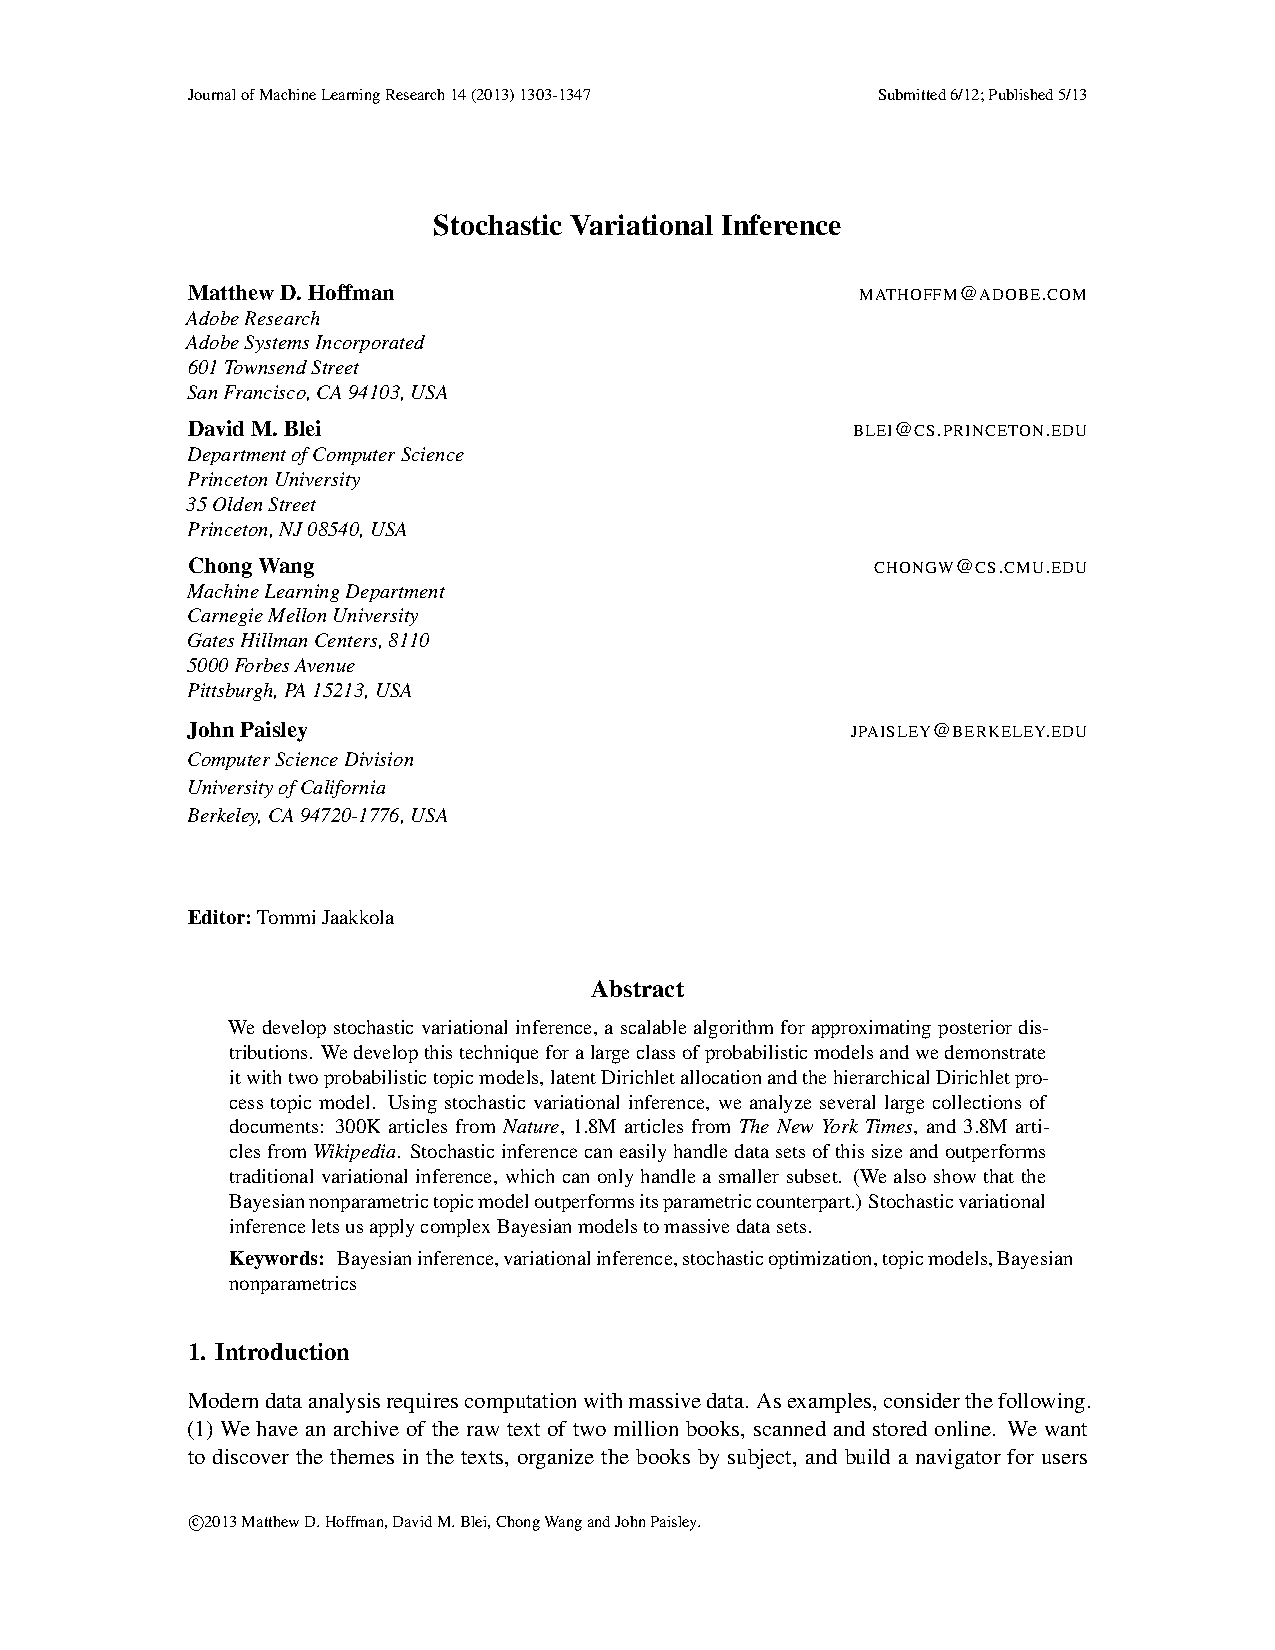
\includegraphics[trim={0cm 15cm 0 0},clip,width=\textwidth]{Papers/svi.pdf}
%     }
%   }
%   \only<2>{
%     \frametitle{or that one}
%     \fbox{
%       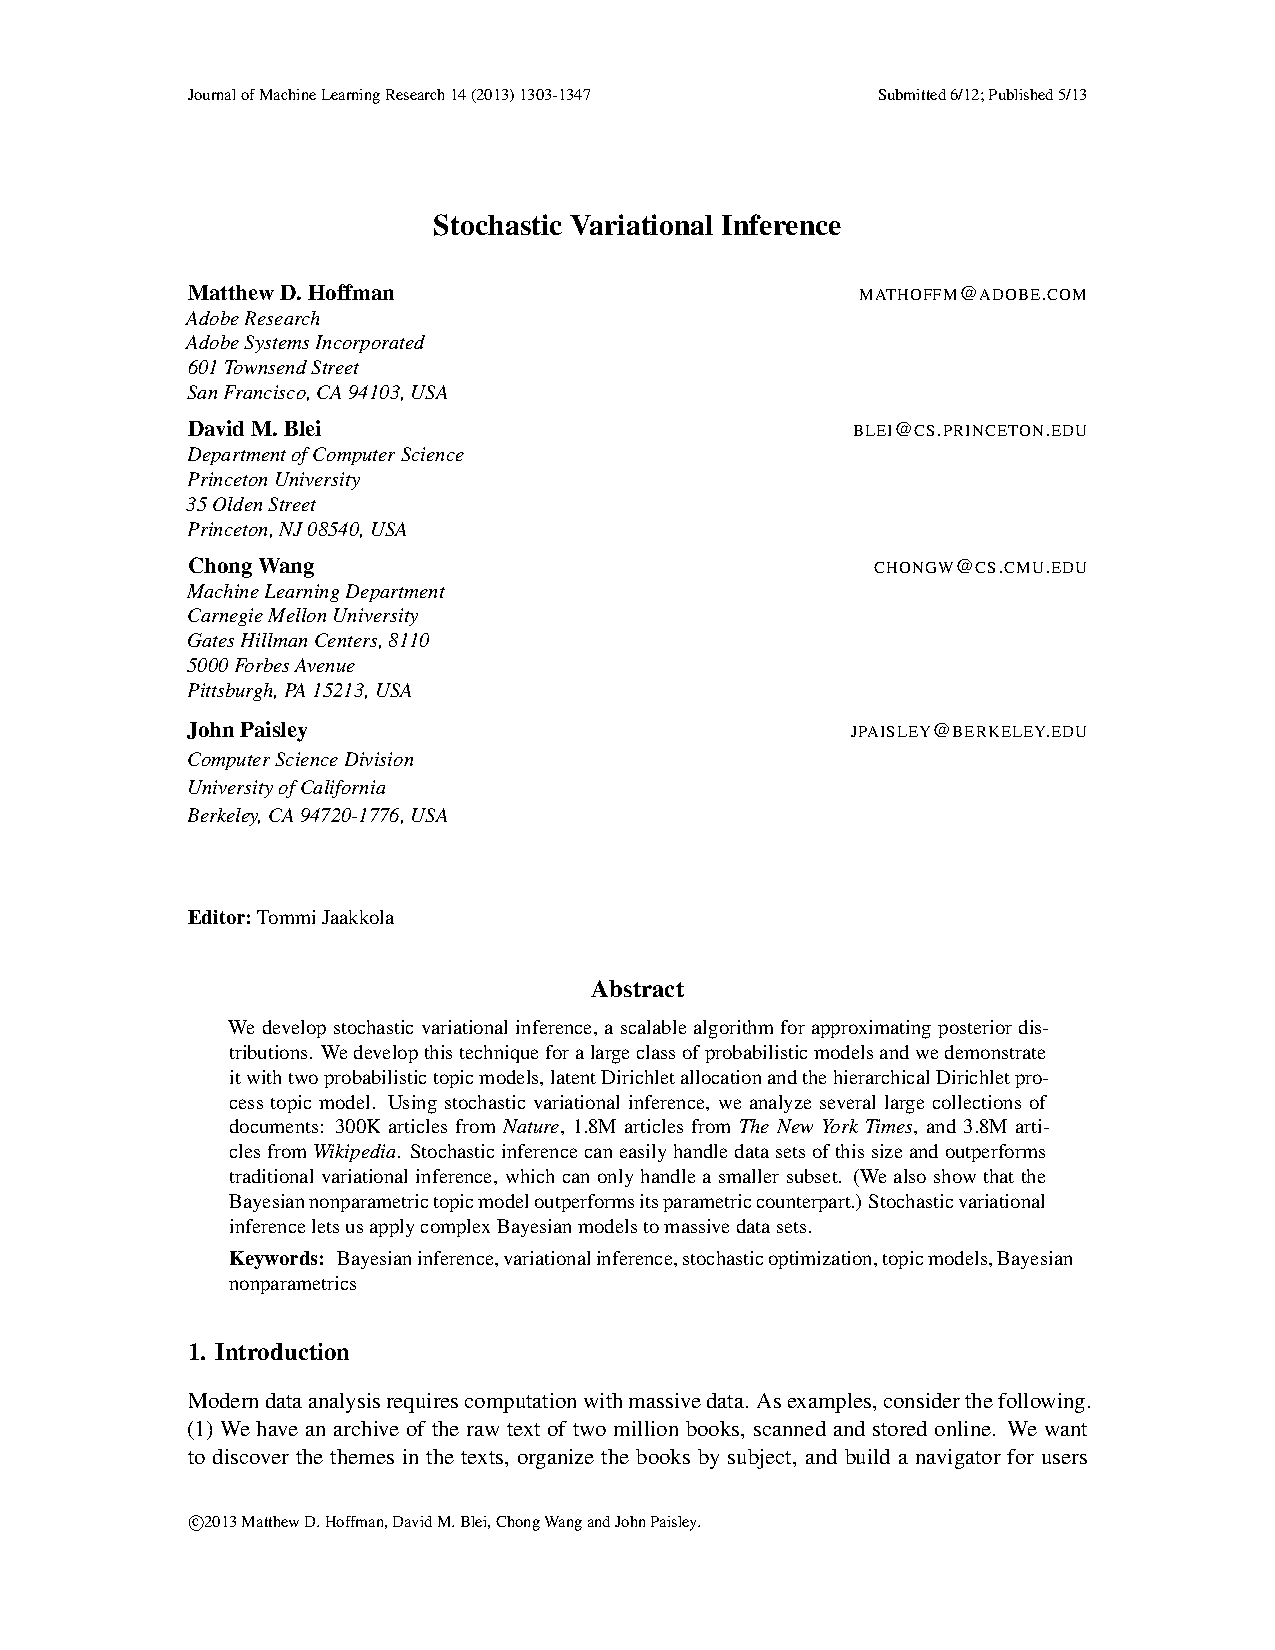
\includegraphics[trim={0cm 0 0 15cm},clip,width=\textwidth]{Papers/svi.pdf}
%     }
%   }
%   \end{frame}
  
  \begin{frame}
  \frametitle{Outline}
  \tableofcontents
  \end{frame}
  
  % \section{A data-driven definition}
  % \begin{frame}
  %   \frametitle{Bayesian keywords in NeurIPS abstracts, up to 2016}
  %   \begin{figure}
  %     \subfigure[``Bayesian" at NeurIPS]{
  %     \includegraphics[width=\twofig]{Figures/bayesianPapersNIPS.pdf}
  %     \label{f:papers:BayesianNeurIPS}
  %     }
  %     \subfigure[``Neural net" at NeurIPS]{
  %     \includegraphics[width=\twofig]{Figures/neuralPapersNIPS.pdf}
  %     \label{f:papers:NNNeurIPS}
  %     }
  %     \label{f:papers}
  %     %\caption{Trends for papers appearing in JMLR and at NeurIPS, up to 2016.}
  % \end{figure}
  % \end{frame}
  
  % \begin{frame}
  %   \frametitle{Topics automatically extracted from 1000+ ``Bayesian" abstracts}
  %   \begin{figure}
  %     \footnotesize
  %     \begin{tabular}{|l|}
  %     \hline
  %       \textcolor{vert}{model models data process latent Bayesian Dirichlet hierarchical nonparametric inference}\\
  %       features learn problem different knowledge learning image object example examples\\
  %       method neural Bayesian using linear state based kernel approach model\\
  %       belief propagation nodes local tree posterior node nbsp given algorithm\\
  %       learning data Bayesian model training classification performance selection prediction sets\\
  %       \textcolor{bleu}{inference Monte Carlo Markov sampling variational time algorithm MCMC approximate}\\
  %       function optimization algorithm optimal learning problem gradient methods bounds state\\
  %       learning networks variables structure network Bayesian EM paper distribution algorithm\\
  %       \textcolor{magenta}{Bayesian gaussian prior regression non estimation likelihood sparse parameters matrix}\\
  %       model information Bayesian human visual task probability sensory prior concept\\
  %     \hline
  %     \end{tabular}
  %     \caption{Topics extracted by stochastic variational latent Dirichlet allocation, using {scikit-learn} \citep{sklearn11}.
  %     \label{f:bayesianTopics}}
  %     \end{figure}
  % \end{frame}
  
  \section{A warmup: Estimation in regression models}
  
  % \begin{frame}{A recap on probabilistic graphical models \citep[Section 10.5]{Mur12}}
  %   \begin{itemize}
  %     \item PGMs (aka ``Bayesian" networks) represent the dependencies in a joint distribution $p(s)$ by \un{a directed graph $G=(E,V)$}.
  %     \item Two important properties:
  %     $$
  %     p(s) = \prod_{v\in V} p(s\vert s_{\text{pa(v)}}) \qquad\text{and}\qquad
  %     s_v \perp s_{nd(v)\setminus pa(v)} \vert s_{pa(v)}.
  %     $$
  %   \end{itemize}
  %   \blank
  % \end{frame}
  
  
  \begin{frame}{Inference in regression models}
  \vspace{-1.5cm}
  \begin{flushright}
    \includegraphics[width=\threefig]{Figures/fisher.jpg}
  \end{flushright}
  \vfill 
  \end{frame}
  
  \begin{frame}{Inference in regression models}
    \vspace{-1.5cm}
    \begin{flushright}
      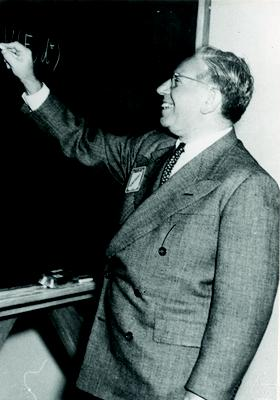
\includegraphics[width=\threefig]{Figures/wald2}
    \end{flushright}
    \vfill 
  \end{frame}
  
  \begin{frame}{Inference in regression models}
    \vspace{-1.5cm}
    \begin{flushright}
      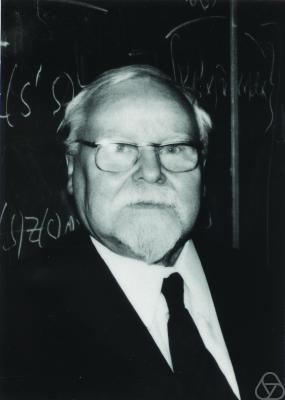
\includegraphics[width=\threefig]{Figures/tykhonov.jpg}
    \end{flushright}
    \vfill 
  \end{frame}
  
  \begin{frame}{Inference in regression models}
    \vspace{-1.5cm}
    \begin{flushright}
      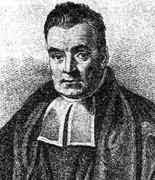
\includegraphics[width=\threefig]{Figures/bayes}
    \end{flushright}
    \vfill 
  \end{frame}
  
  \begin{frame}{Inference in regression models}
  \end{frame}
  

\section{ML as data-driven decision-making}
% \begin{frame}{Abraham Wald (1902--1950)}
%   \centering
%   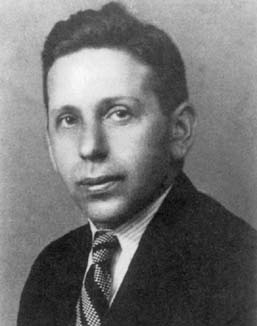
\includegraphics[width=\twofig]{\figdir/wald.jpg}
% \end{frame}

\begin{frame}{Describing a decision problem under uncertainty}
\begin{itemize}
  \vfill\item A state space $\cS$,\\
  \un{Every quantity you need to consider to make your decision.}
  \vfill\item Actions $\cA \subset \cF(\cS, \cZ)$,\\
  \un{Making a decision means picking one of the available actions.}
  \vfill\item A reward space $\cZ$,\\
  \un{Encodes how you feel about having picked a particular action.}
  \vfill\item A loss function $L:\cA\times \cS \rightarrow \mathbb{R}_+$.\\
  \un{How much you would suffer from picking action $a$ in state $s$. 
  % It is also customary to first define a utility $u:\cZ\rightarrow \mathbb{R}_+$, and then let
  % $$ L(a,s) = \sup_{a'\in\cA} u\big(a'(s)\big) - u\big(a(s)\big) \in\mathbb{R}_+.$$
  }
\end{itemize}
\end{frame}

\begin{frame}{Classification as a decision problem}
\begin{itemize}
\item $\cS = \un{\cX^n\times\cY^n}\times \cX\times \cY$, i.e. $s = (x_{1:n}, y_{1:n}, x, y)$.
\item $\cZ = \{0,1\}$.
\item $\cA = \{a_g: s\mapsto 1_{y\neq g(x; \un{x_{1:n}, y_{1:n}})}, \quad g\in\mathcal{G}\}$.
\item $L(a_g,s) = 1_{y\neq g(x; \un{x_{1:n}, y_{1:n}})}$.
\end{itemize}
\vfill
\begin{block}{PAC bounds; see e.g. \citep{ShBe14}}
Let $(x_{1:n},y_{1:n})\sim \mathbb{P}^{\otimes n}$, and independently $(x,y)\sim \mathbb{P}$, we want an algorithm $g(\cdot; x_{1:n}, y_{1:n})\in\mathcal G$ such that if $n\geq n(\delta,\epsilon)$,
$$
\un{\mathbb{P}^{\otimes n}}\left[\mathbb{E}_{(x,y)\sim \mathbb P} L(a_g,s) \leq \epsilon\right] \geq 1-\delta.
$$
\end{block}\end{frame}

\begin{frame}{Regression as a decision problem}
  \begin{itemize}
  \item $\cS = $
  \item $\cZ = $
  \item $\cA = $
  \item
  \end{itemize}
  \blank
\end{frame}

\begin{frame}{Estimation as a decision problem}
  \begin{itemize}
  \item $\cS = $
  \item $\cZ = $
  \item $\cA = $
  \item
  \end{itemize}
  \blank
\end{frame}

\begin{frame}{Clustering as a decision problem}
  \begin{itemize}
    \item $\cS = $
    \item $\cZ = $
    \item $\cA = $
    \item
    \end{itemize}
    \blank
  \end{frame}

% Regression, classification, estimation, dimensionality reduction, clustering, topic modelling as a more complex hidden variable model: gives states and losses, maybe state the main non-Bayesian solution.

\section{Subjective expected utility}
% State the principle, insist on the choice of p, comment on BDA.
% Recap on graphical models
% List all previous examples and show a graphical model and the Bayes action.
% Solve a few examples, link with non-Bayesian solutions like regularized regression. Horseshoe?
% Confront with preconceived ideas on BML. Insist that on top of being a general, interpretable principle, SEU is usually good for non-Bayesians too: BvM, smaller MSE, PAC-Bayes (to come). Moreover, philosophical support (also to come in lecture on foundations).
\begin{frame}{SEU is what defines the Bayesian approach}
\begin{block}{The subjective expected utility principle}
\begin{enumerate}
\item \un{Choose} $\cS, \cZ, \cA$ and a loss function $L(a,s)$,
\item \un{Choose} a distribution $p$ over $\cS$,
\item Take the the corresponding \un{Bayes action}
\begin{equation}
a^\star \in \argmin_{a\in\mathcal{A}} \mathbb{E}_{s\sim p} L(a,s).
\label{e:seu}
\end{equation}
\end{enumerate}
\end{block}
\vfill

\begin{block}{Corollary: minimize the posterior expected loss}
Now partition $s=(s_{\text{obs}}, s_{\text{u}})$, then 
$$ a^\star \in \argmin_{a\in\mathcal{A}} \mathbb{E}_{s_{\text{obs}}} \mathbb{E}_{s_{\text{u}}\vert s_{\text{obs}}} L(a,s).$$
In ML, $\cA = \{a_g\}$, with $g = g(s_\text{obs})$, so that
\eqref{e:seu} is equivalent to $a^\star = a_{g^\star}$, with
$$
g^\star (s_\text{obs}) \triangleq \argmin_{g} \un{\mathbb{E}_{s_{\text{u}}\vert s_{\text{obs}}} L(a,s)}.$$
\end{block}
\end{frame}

\section{Specifying joint models}
\begin{frame}{A recap on probabilistic graphical models 1/2}
  \begin{itemize}
    \item PGMs (aka ``Bayesian" networks) represent the dependencies in a joint distribution $p(y)$ by \un{a directed graph $G=(E,V)$}.
    \item Two important properties:
    $$
    p(y) = \prod_{v\in V} p(y\vert y_{\text{pa(v)}}) \qquad\text{and}\qquad
    y_v \perp y_{nd(v)} \vert y_{pa(v)}.
    $$
    \blank
  \end{itemize}
  \blank
\end{frame}

\begin{frame}{A recap on probabilistic graphical models 2/2}
  \begin{itemize}
    \item Also good to know how to determine whether $A\perp B\vert C$; see \citep[Section 10.5]{Mur12}.
  \end{itemize}
  \centering
  \only<1>{
    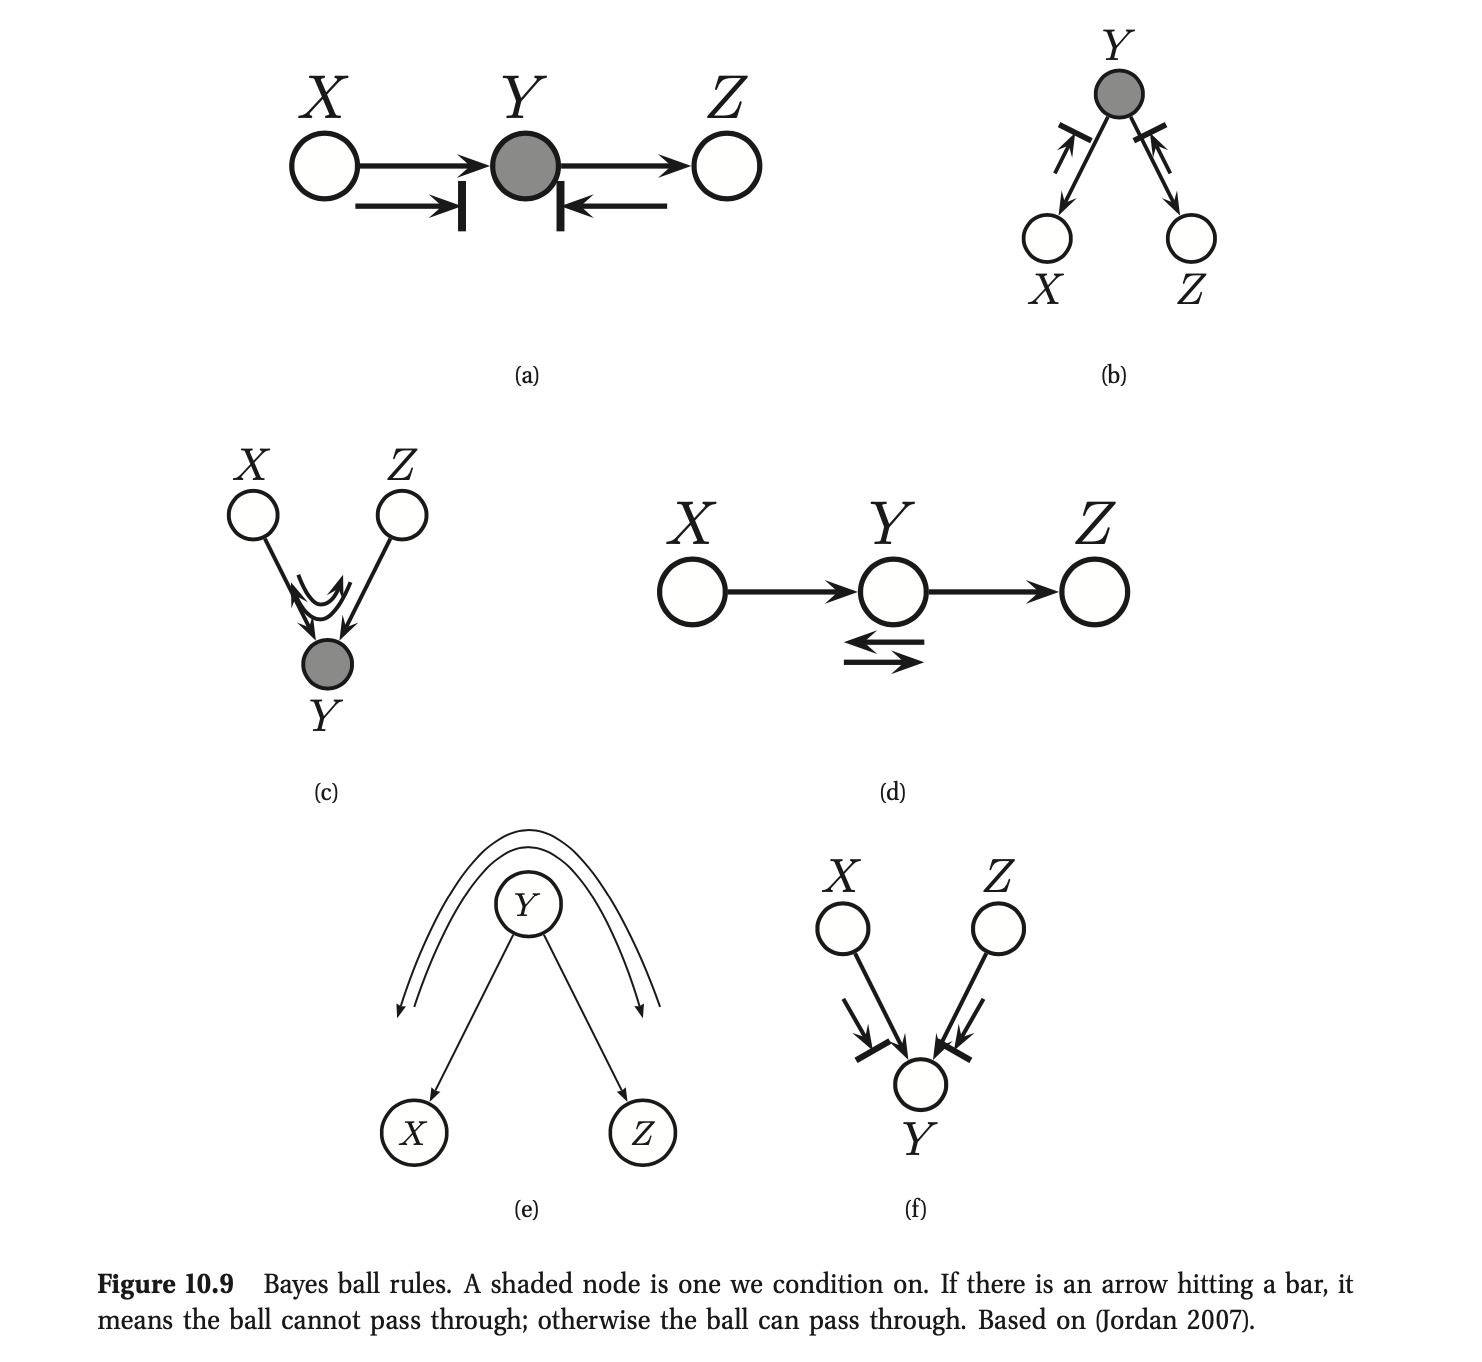
\includegraphics[width=.7\textwidth]{Figures/bayes_ball_1}
  }
  \only<2>{
    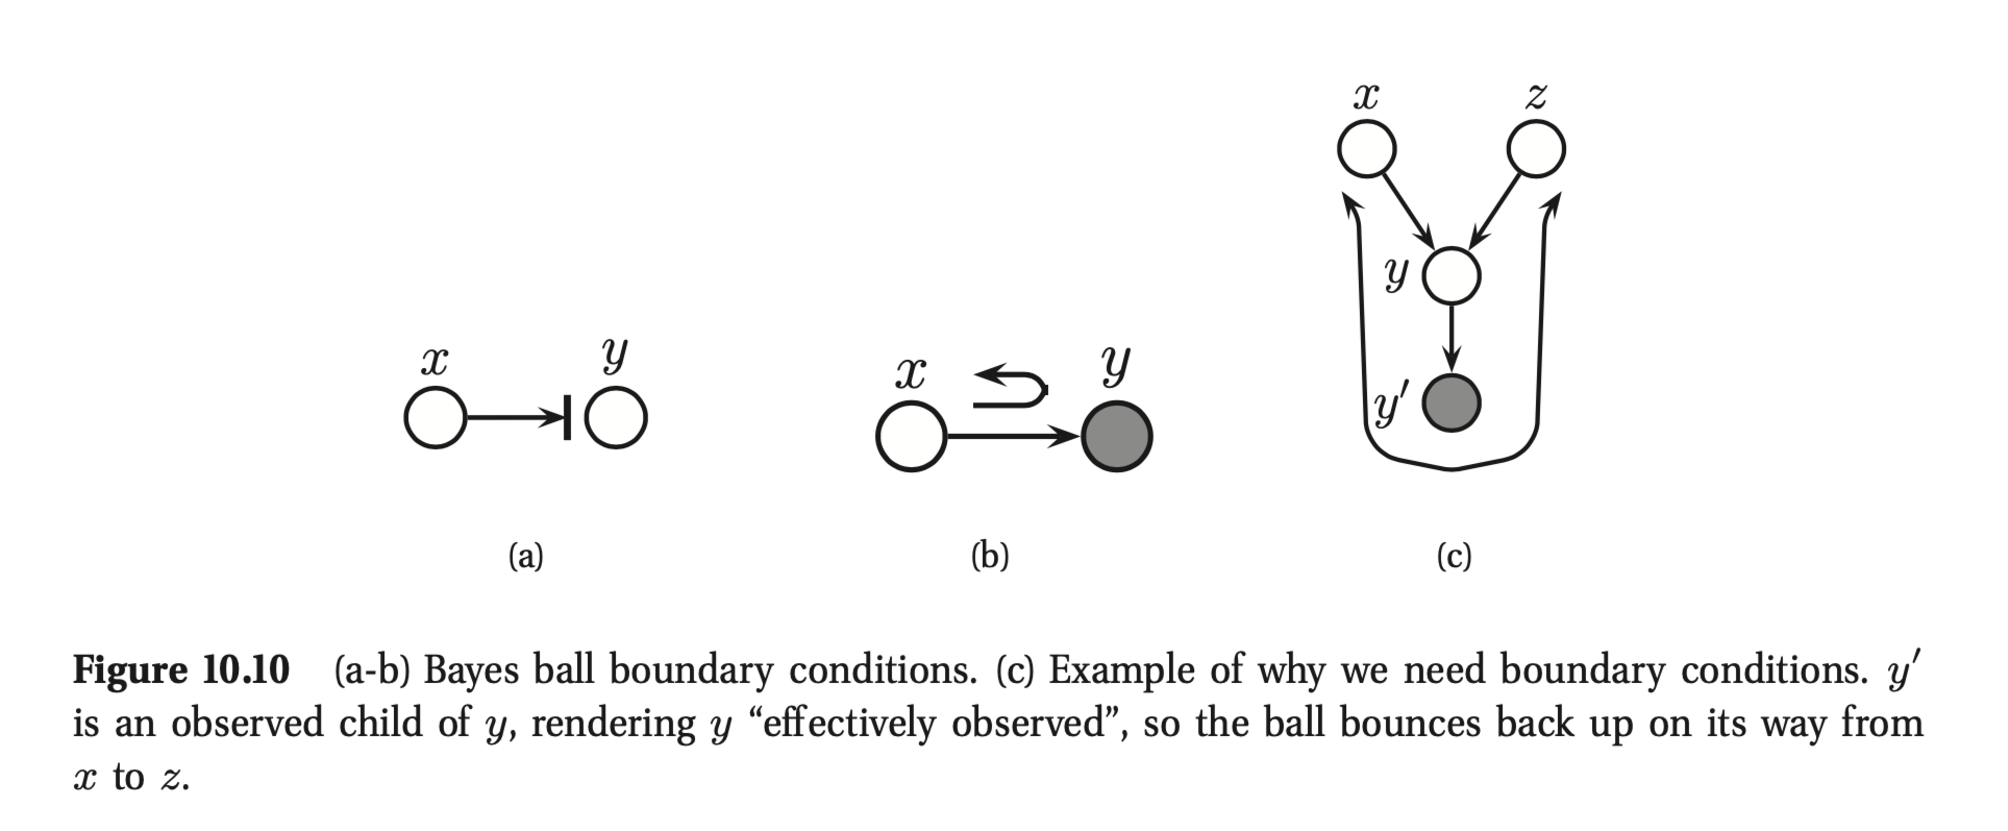
\includegraphics[width=.8\textwidth]{Figures/bayes_ball_2}
  }
  \only<3>{
    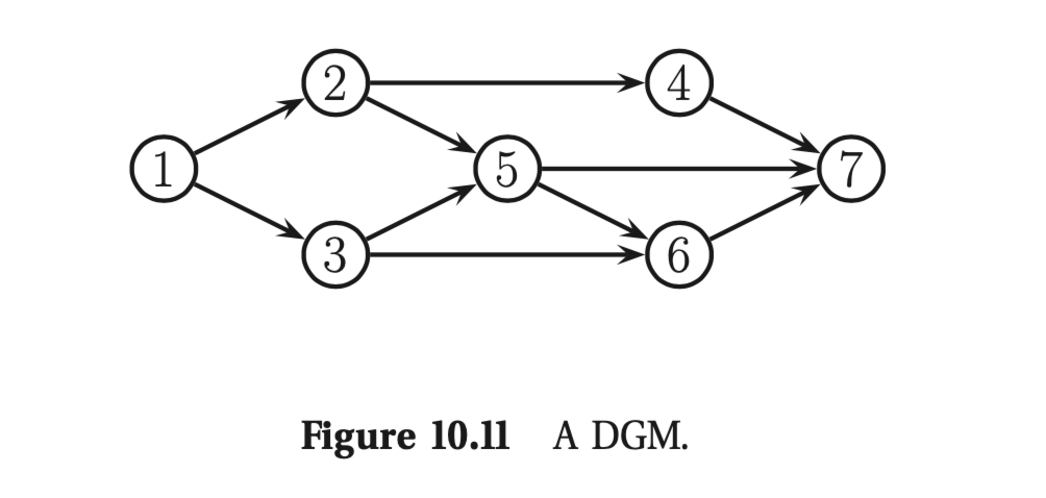
\includegraphics[width=.8\textwidth]{Figures/bayes_ball_3}
    \begin{itemize}
      \item Check that $x_2\perp x_6\vert x_5,x_1$, but that $x_2\not\perp x_6\vert x_5,x_1,x_7$.
    \end{itemize}
    }

\end{frame}


\begin{frame}{Estimation as a decision problem: point estimates}
\end{frame}

\begin{frame}{Estimation as a decision problem: credible intervals}
\end{frame}

\begin{frame}{Choosing priors (see Exercises)}
\end{frame}

\begin{frame}{Classification as a decision problem}
\end{frame}

\begin{frame}{Regression as a decision problem 1/2}
% Exercise: Gaussian-Gaussian model, smaller MSE as an example of having good frequentist properties
\end{frame}

\begin{frame}{Regression as a decision problem 2/2}
% Exercise: Gaussian-Gaussian model, smaller MSE as an example of having good frequentist properties
\end{frame}

\begin{frame}{Dimensionality reduction as a decision problem}
\end{frame}

\begin{frame}{Clustering as a decision problem}
\end{frame}

\begin{frame}{Topic modelling as a decision problem}
\end{frame}

% \begin{frame}{Image denoising as a decision problem}
% \begin{figure}
% \includegraphics[width=\textwidth]{Figures/denoising.png}
% \caption{Taken from \citep[Chapter 21]{Mur12}}
% \end{figure}
% \blank
% \end{frame}

\section{50 shades of Bayes}
% prior should not depend on the data, then advisable to study the effect of the prior after the analysis is done.
% prior should be "non-informative", but then depends on data
% we prefer MAP so prior is only there to regularize -> mainly for computational convenience.
% Sometimes we can turn the ``Bayesianness knob". Example of sparse regression and the horseshoe prior.
\begin{frame}{50 shades of Bayes}
  \begin{alertblock}{An issue (or is it?)}
    Depending on how they interpret and how they implement SEU, you will meet many types of Bayesians (46656, according to Good).
  \end{alertblock}
\begin{block}{A few divisive questions}
\begin{itemize}
\item Using data or the likelihood to choose your prior; see Lecture \#5.
\item Using MAP estimators for their computational tractability, like in inverse problems
$$ \hat x_\lambda \in \argmin \Vert y- Ax\Vert + \lambda\Omega(x).$$
\item When and how should you revise your model (likelihood or prior)?
\item MCMC vs variational Bayes (more in Lectures \#2 and \#3)
\end{itemize}
\end{block}
\end{frame}

\section*{References}
\setbeamertemplate{bibliography item}[text]%,
\begin{frame}[allowframebreaks]
\frametitle{References}
\small
\printbibliography
\normalsize
\end{frame}

\end{document}

% trail junk

\section{The what}

\subsection{Typical statistical problems}
\begin{frame}
\frametitle{Typical jobs for statisticians}
\begin{block}{Estimation}
\begin{itemize}
\item You have data $x_1,\dots,x_n$ that you assume drawn from $p(x_1,\dots,x_n\vert \theta^\star)$, with $\theta^\star\in\mathbb{R}^d$.
\item You want \un{an estimate $\hat{\theta}(x_1,\dots,x_n)$} of $\theta^\star\in\mathbb{R}^d$.
\end{itemize}
\end{block}
\uncover<2>{
\begin{block}{Confidence regions}
  \begin{itemize}
  \item You have data $x_1,\dots,x_n$ that you assume drawn from $p(x_1,\dots,x_n\cdot\vert \theta^\star)$, with $\theta^\star\in\mathbb{R}^d$.
  \item You want \un{a region $A(x_1,\dots,x_n)\subset \mathbb{R}^d$} and make a statement that $\theta\in A(x_1,\dots,x_n)$ with some certainty.
  \end{itemize}
\end{block}
}
\end{frame}

\subsection{Statistical decision theory}
\begin{frame}
\frametitle{Statistical decision theory\footcite{Wal50}}
\begin{figure}
  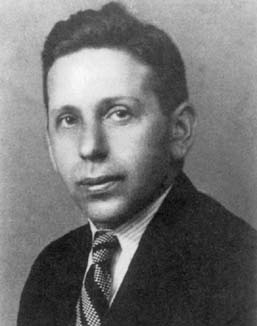
\includegraphics[width=\threefig]{\figdir/wald.jpg}
  \caption{Abraham Wald (1902--1950)}
\end{figure}
\end{frame}

\begin{frame}
\frametitle{Statistical decision theory}
\begin{itemize}
\item Let $\Theta$ be the ``states of the world", typically the space of parameters of interest.
\item Decisions are functions $d(x_1,\dots,x_n)\in \mathcal{D}$.
\item Let $L(d,\theta)$ denote the loss of making decision $d$ when the state of the world is $\theta$.
\item Wald defines the risk of a decision as
  $$ R(d,\theta) = \int L(d,\theta) p(x_{1:n}\vert \theta) \un{dx_{1:n}}.$$
\item Wald says $d_1$ is a \un{better} decision than $d_2$ if
\begin{equation}
  \un{\forall \theta\in\Theta,}\quad L(d_1,\theta)\leq L(d_2,\theta).
\label{e:waldOrder}
\end{equation}
\item $d$ is called \un{admissible} if there is no better decision than $d$.
\end{itemize}
\end{frame}

\begin{frame}
\frametitle{Illustration with a simple estimation problem}
\begin{itemize}
  \item You have data $x_1,\dots,x_n$ that you assume drawn from
  $$p(x_1,\dots,x_n\vert \theta^\star) = \prod_{i=1}^n \cN(x_i\vert\theta^\star,\sigma^2),$$ and you know $\sigma^2$.
  \item You \un{choose} a loss function, say $L(\hat{\theta},\theta) = \Vert \hat{\theta}-\theta\Vert^2.$
  \item You \un{restrict} your decision space to unbiased estimators.
  \item The sample mean $\tilde{\theta}:= n^{-1}\sum_{i=1}^n x_i$ is unbiased, and has minimum variance among unbiased estimators.
  \item Since $$R(\tilde\theta,\theta) = \text{Var}\tilde\theta,$$ $\tilde{\theta}$ is the \un{best decision} you can make in Wald's framework.
\end{itemize}
\end{frame}

\begin{frame}
  \frametitle{Wald's view of frequentist estimation}
  \begin{block}{Estimation}
  \begin{itemize}
  \item You have data $x_1,\dots,x_n$ that you assume drawn from $p(x_1,\dots,x_n\vert \theta^\star)$, with $\theta^\star\in\mathbb{R}^d$.
  \item You want \un{an estimate $\hat{\theta}(x_1,\dots,x_n)$} of $\theta^\star\in\mathbb{R}^d$.
  \end{itemize}
  \end{block}

\begin{exampleblock}{A Waldian answer}
\begin{itemize}
\item Our decisions are estimates $d(x_1,\dots,x_n) = \hat{\theta}(x_1,\dots,x_n)$.
\only<1>{
\item \un{We pick a loss}, say $L(d,\theta) = L(\hat{\theta},\theta) = \Vert \hat{\theta}-\theta\Vert^2$.
\item
If you have an unbiased estimator with minimum variance, then this is \un{the best decision among unbiased estimators}.
}
\only<2>{
\item In general, the loss can be more complex and unbiased estimors unknown/irrelevant.
\item In these cases, you may settle for a \un{minimax estimator}
$$ \hat\theta(x_1,\dots,x_n) = \argmin_d \sup_\theta R(d,\theta).$$
}
\end{itemize}
\end{exampleblock}
\end{frame}

\begin{frame}
\frametitle{Wald's is only \emph{one} view of frequentist statistics...}
\begin{itemize}
\item On estimation, some would argue in favour of the maximum likelihood \footcite{Sti07}.
\end{itemize}
\begin{figure}
  \includegraphics[width=\threefig]{\figdir/fisher.jpg}
  \caption{Ronald Fisher (1890--1962)}
\end{figure}
% In a sense, MLE is a limiting case of Wald's approach, but not clean
\end{frame}

\begin{frame}
\frametitle{... but bear with me, since it is predominant in machine learning}
For instance, supervised learning is usually formalized as
\begin{equation}
g^\star = \argmin_g \mathbb{E}L(y,g(x)).
\label{e:learning}
\end{equation}
which you approximate by
$$ \hat{g} = \argmin_g \sum_{i=1}^n L(y_i,g(x_i)) + \text{penalty}(g),$$
while trying to control the excess risk
$$ \mathbb{E}L(y,\hat g(x)) - \mathbb{E}L(y,g^\star(x)).$$
\end{frame}


\begin{frame}
  \frametitle{Wald's view of frequentist confidence regions}
  \begin{block}{Confidence regions}
    \begin{itemize}
    \item You have data $x_1,\dots,x_n$ that you assume drawn from $p(x_1,\dots,x_n\cdot\vert \theta^\star)$, with $\theta^\star\in\mathbb{R}^d$.
    \item You want \un{a region $A(x_1,\dots,x_n)\subset \mathbb{R}^d$} and make a statement that $\theta\in A(x_1,\dots,x_n)$ with some certainty.
    \end{itemize}
  \end{block}

\begin{exampleblock}{A Waldian answer}
\begin{itemize}
\item Our decisions are subsets of $\mathbb{R}^d$: $d(x_{1:n}) = A(x_{1:n})$.
\item A common loss is $L(d,\theta) = L(A,\theta) = 1_{\theta\notin A} + \gamma \vert A\vert $.
\item So you want to find $A(x_{1:n})$ that minimizes
$$ L(A,\theta) = \int \left[1_{\theta^\star\notin A} p(x_{1:n}\vert\theta^{\star}) + \gamma \vert A\vert\right] dx_{1:n} .$$
\end{itemize}
\end{exampleblock}
\end{frame}

\begin{frame}
\frametitle{Illustration with a simple confidence interval problem}
\begin{itemize}
  \item You have data $x_1,\dots,x_n$ that you assume drawn from
  $$p(x_1,\dots,x_n\vert \theta^\star) = \prod_{i=1}^n \cN(x_i\vert\theta^\star,\sigma^2).$$
  \item You \un{choose} a loss function, say $L(A,\theta) = 1_{\theta\notin A} + \gamma \vert A\vert $.
  \item You \un{restrict} your decisions to intervals centered around the sample mean $\tilde\theta$.
  \item Since $\frac{\theta - \tilde\theta}{\sigma/\sqrt{n}} \sim \cN(0,1)$,
  we know \unn{(exercise)} that for $$\tilde{A} := [\tilde\theta - k\sigma/\sqrt{n}, \tilde\theta + k\sigma/\sqrt{n}],$$
  it comes
  $$ R(A, \theta) = \mathbb{P}(\vert\cN(0,1)\vert \geq k) + \frac{2\gamma k\sigma}{\sqrt{n}}.$$
  \item All is left to do is choose $k$.
  \item Textbook examples bypass the need for $\gamma$: they fix $\alpha>0$ and find the smallest $k$ such that $\mathbb{P}(\vert\cN(0,1)\vert \geq k)\leq \alpha$.
\end{itemize}
\end{frame}

\begin{frame}
\frametitle{Summary so far}
% Maybe introduce a classification example here
\begin{itemize}
\item Waldian frequentists measure risks as expectations w.r.t. the data-generating process.
$$ R(d,\theta) = \int L(d(x_{1:n}),\theta) p(x_{1:n}\vert \theta)dx_{1:n}$$
\item One major difficulty is that the risk remains a function of $\theta$.
\item Without additional structure (unbiasedness, Gaussianity, etc.), it is difficult to go beyond minimax rules.
\end{itemize}
\begin{block}{Idea}
What if we introduced a distribution on $\Theta$, and tried to minimize
\begin{align*}
  r(d) &= \int R(d,\theta) p(\theta) \un{d\theta}\\
   &= \int\left[\int  L(d(x_{1:n}),\theta) p(x_{1:n}\vert \theta)dx_{1:n}\right]p(\theta)\un{d\theta}
\end{align*}
\end{block}
\end{frame}

\begin{frame}
\frametitle{From expected frequentist loss to posterior expected loss}
\begin{align*}
  r(d) &= \int R(d,\theta) p(\theta) \un{d\theta}\\
   &= \int\left[\int  L(d(x_{1:n}),\theta) p(x_{1:n}\vert \theta)dx_{1:n}\right]p(\theta)\un{d\theta}\\
   &\textcolor{red}{=} \int\left[\int  L(d(x_{1:n}),\theta) p(x_{1:n}\vert \theta)p(\theta)\un{d\theta} \right]dx_{1:n}\\
   &= \int\left[\int  L(d(x_{1:n}),\theta) \unn{\frac{p(x_{1:n}\vert \theta)p(\theta)}{p(x_{1:n})}}\un{d\theta} \right] p(x_{1:n}) dx_{1:n}\\
   &= \int\left[\int  L(d(x_{1:n}),\theta) \unn{p(\theta\vert x_{1:n})}\un{d\theta} \right] p(x_{1:n}) dx_{1:n}
\end{align*}
\end{frame}

\subsection{Posterior expected utility and Bayes rules}
\begin{frame}
\frametitle{Bayesians minimize posterior expected utility}
\begin{block}{The posterior expected utility paradigm: Bayes rules}
Pick $d$ to solve
$$ \argmin_d \int  L(d(x_{1:n}),\theta) p(\theta\vert x_{1:n}) d\theta. $$
\end{block}
\begin{exampleblock}{Bayes rules have good frequentist properties\footcite{PaIn09}}
\begin{itemize}
\item Under general conditions, Bayes decision rules are admissible, all admissible rules are limits of Bayes rules.
\item Bayes rules with ``least favourable priors" are minimax.
\end{itemize}
\end{exampleblock}
\end{frame}

\begin{frame}
  \frametitle{Illustration with a simple estimation problem}
  \begin{itemize}
    \item You have data $x_1,\dots,x_n$ that you assume drawn from
    $$p(x_1,\dots,x_n\vert \theta^\star) = \prod_{i=1}^n \cN(x_i\vert\theta^\star,\sigma^2),$$ and you know $\sigma^2$.
    \item You \un{choose} a loss function, say $L(\hat{\theta},\theta) = \Vert \hat{\theta}-\theta\Vert^2.$
    \item You \un{choose} a prior $p$ over $\theta$.
    \item Your Bayes decision minimizes
    $$ \int \Vert\hat{\theta}-\theta\Vert^2 p(\theta\vert x_{1:n})d\theta,$$
    so you pick
    $$ \hat\theta = \int \theta p(\theta\vert x_{1:n}) d\theta.$$
    \item Conceptually, it is simpler. In practice, you need to compute an integral.
  \end{itemize}
  \end{frame}

  \begin{frame}
  \frametitle{Illustration with a simple confidence interval problem}
  \begin{itemize}
    \item You have data $x_1,\dots,x_n$ that you assume drawn from
    $$p(x_1,\dots,x_n\vert \theta^\star) = \prod_{i=1}^n \cN(x_i\vert\theta^\star,\sigma^2).$$
    \item You \un{choose} a loss function, say $L(A,\theta) = 1_{\theta\notin A} + \gamma \vert A\vert $.
    \item You \un{choose} a prior $p$ over $\theta$.
    \item Your Bayes decision minimizes
    $$ \int 1_{\theta\notin A} p(\theta\vert x_{1:n})d\theta + \gamma\vert A\vert,$$
    \item Conceptually, it is simpler. In practice, you need to carefully pick your prior and/or restrict the decision space and/or compute many integrals.
  \end{itemize}
  \end{frame}

% \begin{frame}
%   \frametitle{Again, Wald's view is not universal}
%   \begin{center}
%   \includegraphics[width=\textwidth]{\figdir/stackexchange.png}
%   \end{center}
% \end{frame}

\begin{frame}
  \frametitle{Summary so far}
  \begin{itemize}
    \item Bayes rules fit into Wald's framework.
    \item \un{For a fixed prior}, the Bayesian risk completely orders decision rules.
    \item The \un{key idea} is posterior expected utility.
    \item You can answer most basic statistical questions using this principle: [more examples].
  \end{itemize}
\end{frame}

\begin{frame}
  \frametitle{A recent motivating success}
  \only<1>{
  \fbox{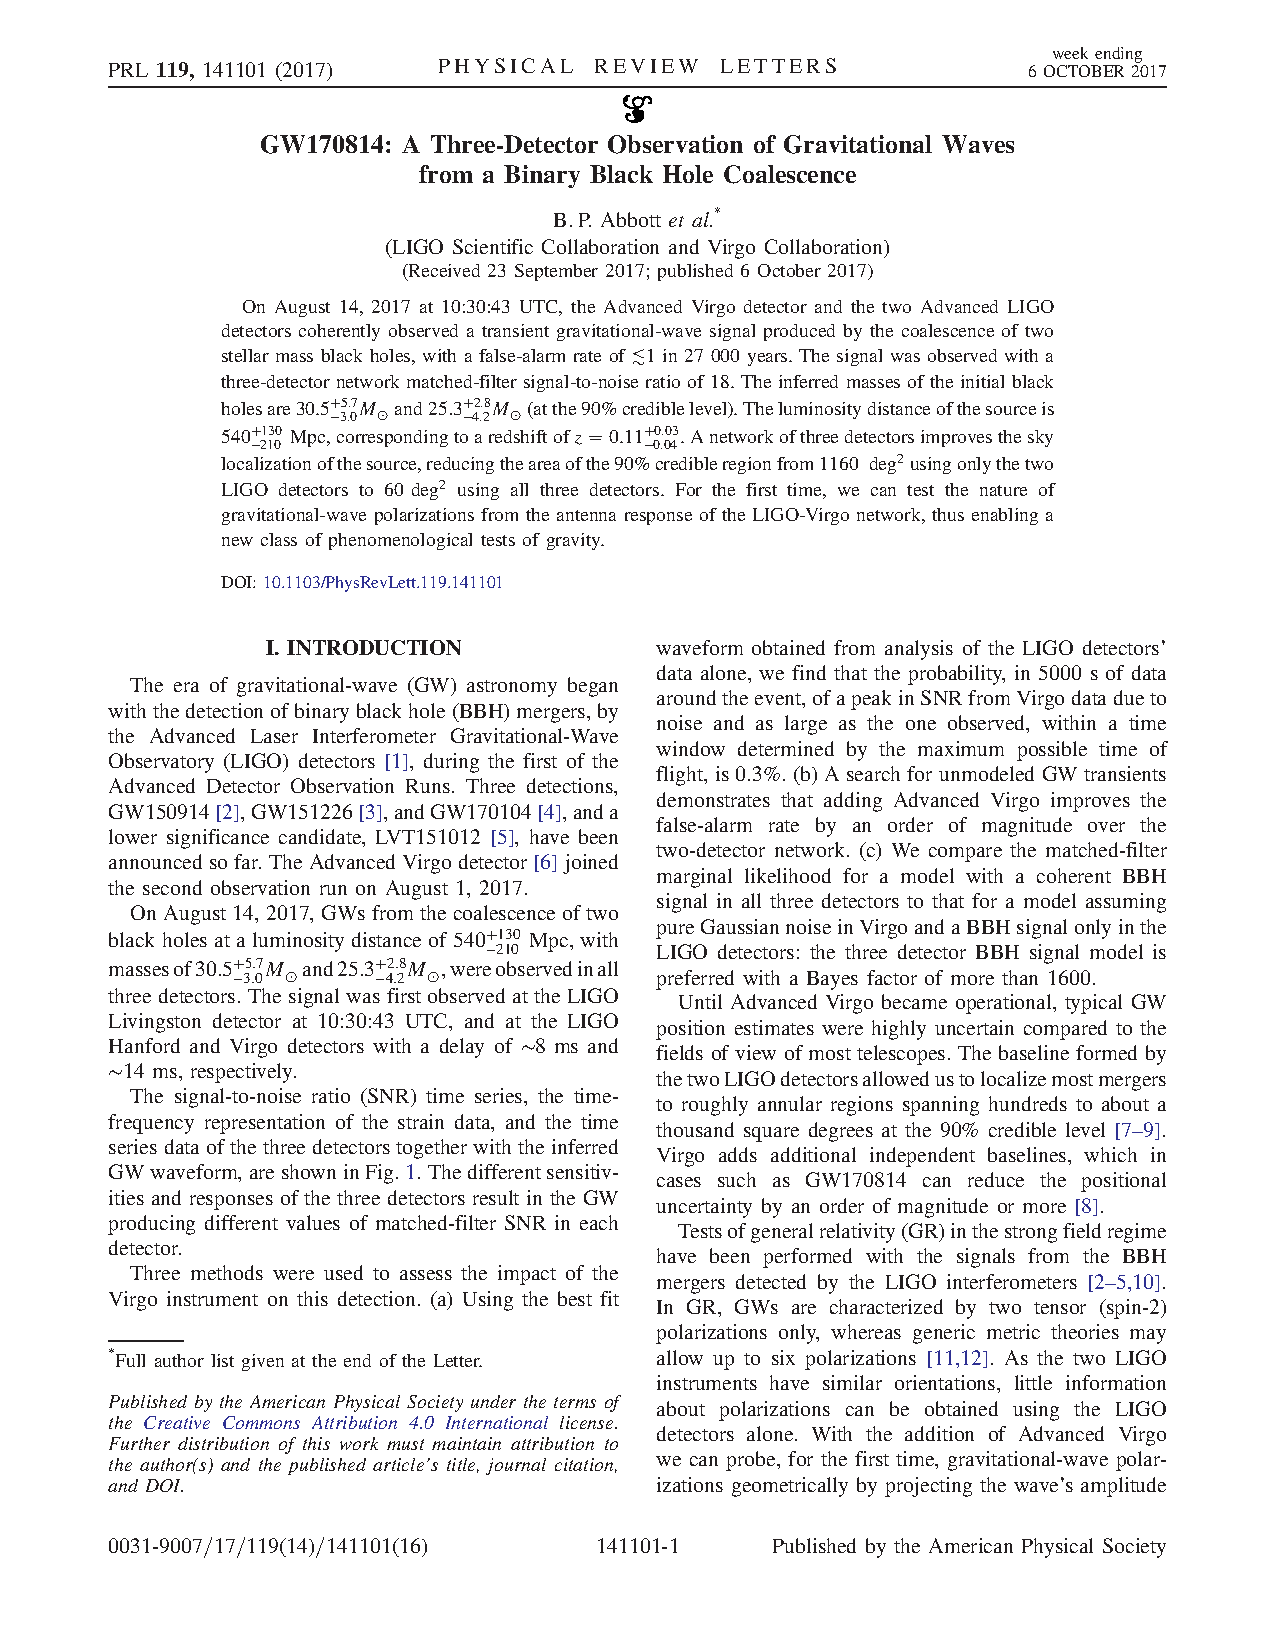
\includegraphics[trim={0 15cm 0 0},clip,width=\textwidth]{Papers/virgo.pdf}}
  }
\end{frame}


\section{The why}
\subsection{The philosophical why}

\begin{frame}
  \frametitle{The subjectivistic viewpoint}
  \begin{itemize}
    \item Top requirement is \un{internal coherence} of decisions.
    \item Favourizes interpreting probability distributions as personal beliefs.
    \begin{figure}
      \centering
      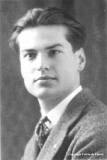
\includegraphics[width=\threefig]{\figdir/deFinetti.jpg}
      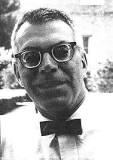
\includegraphics[width=\threefig]{\figdir/savage.jpg}
      \caption{Bruno de Finetti (1906--1985) and L. Jimmie Savage (1917--1971)}
    \end{figure}
  \end{itemize}
\end{frame}

\begin{frame}
  \frametitle{The logical justification}
  \begin{itemize}
    \item Top requirement is to find a version of propositional logic that allows taking into account uncertainty.
    \item Also favourizes interpreting \un{probability distributions as beliefs}, but aims for objective priors.
    \begin{figure}
      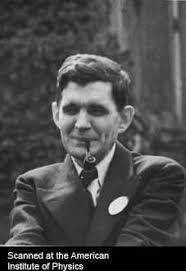
\includegraphics[width=\threefig]{\figdir/cox.jpg}
      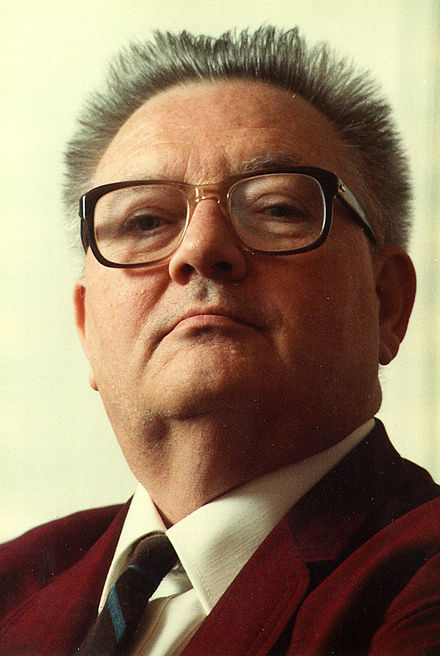
\includegraphics[width=\threefig]{\figdir/jaynes.jpg}
      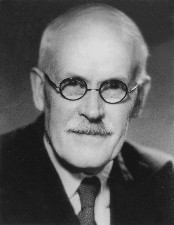
\includegraphics[width=\threefig]{\figdir/jeffreys.jpg}
      \caption{Richart T. Cox (1898--1991), Edwin T. Jaynes (1917--1971), and Harold Jeffreys (1891--1989)}
    \end{figure}
  \end{itemize}
\end{frame}

\begin{frame}
  \frametitle{The hybrid view\footcite{Rob07}}
  \begin{itemize}
    \item The starting point is posterior expected utility, loosely justified by Wald's theory.
    \item It is simple, widely applicable, has good frequentist properties.
    \item It satisfies the \un{likelihood principle}.
    \item It is easy to interpret: beliefs are
    \begin{itemize}
      \item represented by probabilities,
      \item updated using Bayes' rule,
      \item integrated when making decisions.
    \end{itemize}
    \item It is easy to communicate your uncertainty
    \begin{itemize}
      \item Simply give your posterior.
      \item When making a decision, make sure that the priors of everyone involved would yield the same decision.
    \end{itemize}
  \end{itemize}
\end{frame}

\subsection{The practical why}
\begin{frame}
  \frametitle{Practical advantages of posterior expected utility}
  \begin{itemize}
    \item Conceptually answers all ML problems.
    \item Suits all applications \un{where quantifying uncertainty is vital vs computational complexity}: all basic sciences, health, even one-shot commercial decisions.
    \item We \un{never} invoked any large-sample argument, so suits all sizes of datasets.
  \end{itemize}
\end{frame}


\section{The how}
\subsection{Conjugacy}
\begin{frame}
\frametitle{Conjugacy}
\begin{itemize}
\item Say we have a linear regression problem
$$ y_i = f(x_i) + \epsilon_i,$$
$f(x) = \theta^T x$, $\epsilon_i$ i.i.d. Gaussians $\cN(0,\sigma^2)$.
\item If we choose $p(\theta)\sim\cN(0,\Sigma)$, then \unn{(exercise)}
\begin{align*}
  p(\theta\vert (x,y)_{1:n}) &\propto p( (x,y)_{1:n}\vert \theta)p(\theta)\\
  &= \cN(\un{\sigma^{-2}A^{-1}X\by}, A^{-1}),
\end{align*}
where $A=\sigma^{-2}X^TX + \Sigma^{-1}$.
\item If the loss is not too complicated, then integrals are easy. For instance, prediction with $L^2$ loss is simple:
\only<3>{
$$
\argmin_{y_\star} \int \Vert y_\star - \un{f(x_\star)}\Vert^2 p(\theta\vert(x,y)_{1:n})d\theta
$$
}
\only<4>{
$$
\argmin_{y_\star} \int \Vert y_\star - \un{\theta^T x_\star}\Vert^2 p(\theta\vert(x,y)_{1:n})d\theta
$$
}
\only<5>{
$$
\hat y_\star := \un{\sigma^{-2} x_\star^T A^{-1}X\by}.
$$
}
\end{itemize}
\end{frame}

\subsection{Monte Carlo methods}
\begin{frame}
\frametitle{Monte Carlo methods}
\begin{itemize}
  \item Sometimes, you're less lucky. Say we're doing logistic regression.
  $$ y_i = \text{Bernoulli}\left[\sigma(f(x_i))\right],$$
  with $f(x) = \theta^T x$, $\sigma(x) = 1/(1+e^{-x})$.
  \item Even if we choose $p(\theta)\sim\cN(0,\Sigma)$,
  \begin{align*}
    p(\theta\vert (x,y)_{1:n}) &\propto p( (x,y)_{1:n}\vert \theta)p(\theta)
    &\
  \end{align*}
  does not have a simple closed form.
  \item We need powerful \un{numerical integration} methods, that is, constructions of nodes $(\theta_i)$ and weights $w_i$ such that
  $$ \int h d\pi \approx \sum_{i=1}^N w_i h(\theta_i).$$
\end{itemize}
\end{frame}

\subsection{Metropolis-Hastings}
\begin{frame}
\frametitle{Metropolis-Hastings}
\begin{algorithm}{$\Algo{MH}\big(\pi(\theta),\, q(\theta'\vert\theta),\,\theta_{0},\, N_{\text{iter}}\big)$}
\Aitem \For $k\setto1$ \To $N_{\text{iter}}$
\uncover<2->{
\Aitem \mt $\theta\setto\theta_{k-1}$
\Aitem \mt $\theta'\sim q(.\vert\theta)$,} \uncover<4->{$u\sim\cU_{(0,1)}$,
}
\uncover<3->{
\Aitem \textcolor{vert}{\unn{}\mt $\alpha =  \frac{\pi(\theta')}{\pi(\theta)}\frac{q(\theta\vert\theta')}
{q(\theta'\vert\theta)}$}}
\uncover<4->{
\Aitem \mt \If $u<\alpha$
\Aitem \mtt $\theta_{k}\setto\theta'$
\mt \algoremark{\unn{Accept}}
\Aitem \mt \Else $\theta_{k}\setto\theta$
\mt \algoremark{\unn{Reject}} \label{ai:acceptanceEnd}
}
\uncover<5->{
\Aitem
\Return $(\theta_{k})_{k=1,\dots,N_{\text{iter}}}$
}\end{algorithm}
\end{frame}

\begin{frame}
\frametitle{The MCMC magic}
\begin{itemize}
\item Under assumptions\footcite{DoMoSt14},
$$
\sqrt{N_{\text{iter}}}\left[\frac{1}{N_{\text{iter}}}\sum_{k=0}^{N_{\text{iter}}}h(\theta_{k})-\int
  h\left(\theta\right)\pi(\theta)d\theta\right]\rightarrow\cN(0,\sigma_{\text{lim}}^{2}(h)),
$$
\item If you choose $q$ carefully, you can hope for a \un{polynomial increase} of the mixing time and $\sigma_{\text{lim}}^{2}(h)$ with $d$.
\item Most MCMC algorithms are instances of Metropolis-Hastings with \un{clever choices of proposal}\footcite{RoCa04}, even the NUTS HMC of Stan and PyMC3.
\item For nice illustrations, check out \url{https://chi-feng.github.io/mcmc-demo/}
\end{itemize}
\end{frame}


\subsection{Variational approximations}
\begin{frame}
\frametitle{Variational approximations}
\begin{itemize}
\item When in a hurry, you can settle for a good approximation to your posterior
$$ \pi(\theta) = p(\theta\vert\bx) \propto p(\bx\vert\theta)p(\theta),$$
say minimize in $q$
\begin{align*}\text{KL}(q, \pi) &= \mathbb{E}_q \log q - \mathbb{E}_q \log p(\theta\vert \bx)\\
  &= -\un{\left[ -\mathbb{E}_q \log q + \mathbb{E}_q \log p(\bx,\theta)\right]} + \log p(\bx).
\end{align*}
\item Equivalently, we can maximize the \un{evidence lower bound (ELBO)}\footcite{BlKuAu17}.
\item Ideally, I would rather cast the choice of $q$ into a Wald-like problem.
\end{itemize}
\end{frame}

\section{In depth with Gaussian processes in ML}

\subsection{From linear regression to GPs}
\begin{frame}
\frametitle{Linear regression}
\begin{itemize}
  \item $ y_i = f(x_i) + \epsilon_i,$ $f(x) = \theta^T x$, $\epsilon_i$ i.i.d. Gaussians $\cN(0,\sigma^2)$.
\item If we choose $p(\theta)\sim\cN(0,\Sigma^2)$, then
\begin{align*}
  p(\theta\vert (x,y)_{1:n}) &\propto p( (x,y)_{1:n}\vert \theta)p(\theta)\\
\only<1>{
&= \unn{\text{[Exercise]}}\\
}
\only<2->{
  &\propto \exp\left[-\frac{\Vert \by-X\theta\Vert^2}{2\sigma^2} - \frac{\theta^T\Sigma^{-1}\theta}{2}\right]\\
  }
\only<3->{
  &\propto \exp\left[\frac{\by^T X\theta}{\sigma^2} - \frac{\theta^T X^T X \theta}{2\sigma^2} - \frac{\theta^T\Sigma^{-1}\theta}{2}\right]\\
  }
\only<4->{
  &\propto \exp\left[-\frac12 \left(\theta-  \sigma^{-2}A^{-1}X\by\right)^T A \left(\theta-  \sigma^{-2}A^{-1}X\by\right)\right]\\
}
\only<5->{
  &= \cN(\un{\sigma^{-2}A^{-1}X\by}, A^{-1}),
}
\end{align*}
where $A=\sigma^{-2}X^TX +\Sigma^{-1}$.
\only<6>{
\item Remember prediction with $L^2$ loss is simple:
$$
\argmin_{y_\star} \int \Vert y_\star - \un{f(x_\star)}\Vert^2 p(\theta\vert(x,y)_{1:n})d\theta = \un{\sigma^{-2} x_\star^T A^{-1}X\by}.
$$
}
\only<7>{
\item Actually, we can even check that
$$
p(f(x_\star) \vert x_\star,(x,y)_{1:n}) = \cN(\un{\sigma^{-2} x_\star^T A^{-1}X\by}, \unn{{x^{\star}}^T A^{-1}x^{\star}}).
$$
}
\end{itemize}
\end{frame}

\begin{frame}
\frametitle{Linear regression with nonlinear features}
\begin{itemize}
\item Replace each $x$ by a vector of features $\phi(x)\in\mathbb{R}^p$:
$$ y_i = f(x_i) + \epsilon_i, \quad i=1,\dots,n,$$
$f(x) = \theta^T \phi(x)$, $\epsilon_i$ i.i.d. Gaussians $\cN(0,\sigma^2)$, $\theta\sim\cN(0,\Sigma)$.
\item Think $\phi(x) = (1,x^1,x^2,x^1 x^2,\dots)$
\item Recall
$$
p(f(x_\star) \vert x_\star,(x,y)_{1:n}) = \cN(\un{\sigma^{-2} \Phi_\star^T A^{-1}\bPhi\by}, \unn{\Phi^{\star} A^{-1}\Phi^{\star}})
$$
where $A=\sigma^{-2}\bPhi^T\bPhi +\Sigma^{-1}$.
\item Requires $p\times p$ inversion.
\item But let $\mathbf{K} = \bPhi\Sigma\bPhi^T$, then can rewrite \unnn{(Exercise)}
$$
p(f(x_\star) \vert (x,y)_{1:n}) = \cN(\un{\mu_\star}, \unn{\sigma_\star^2}),$$
where
\begin{align*}
\mu_\star &= \un{\Phi_\star^T\Sigma\bPhi^T (\bK+\sigma^2 I)^{-1}\by},\\
\sigma_\star^2 &= \unn{\phi_\star\Sigma\phi_\star - \phi_\star^T\Sigma\bPhi^T(\bK+\sigma^2 I)^{-1} \bPhi\Sigma\phi_\star}.
\end{align*}
\end{itemize}
\end{frame}

% Then with features, then with GPs.

\begin{frame}
\frametitle{Gaussian processes}
\begin{itemize}
\item A distribution over a space of functions $f:\mathbb{R}^d\rightarrow\mathbb{R}$.
\begin{block}{Gaussian processes}
If $\forall p\in\mathbb{N}, \forall x_1,\dots,x_p\in\mathbb{R}^d$
$$ \left[f(x_1), \dots, f(x_p)\right]^T \sim \mathcal{N}(\mathbf{m}, \mathbf{K}),$$
where $\mathbf{m} = \left[\mu(x_1), \dots, \mu(x_p)\right]$ and $$\mathbf{K} = ((K(x_i,x_j))),$$
then we say $f\sim GP(\mu,K)$.
\end{block}
\item Unicity is usually easy, existence is tricky.
\item Necessary condition is that all matrices $\mathbf{K}$ are positive definite.
\end{itemize}
\end{frame}

\begin{frame}
\frametitle{Sampling, conditioning and predicting}
See notebook 01 on
\url{https://github.com/rbardenet/bnp-course}
\end{frame}

\subsection{Modeling and learning}
\begin{frame}
\frametitle{Commonly-used kernels}
\includegraphics[width=\textwidth]{Figures/kernels}
\end{frame}

\begin{frame}
\frametitle{Learning}
\begin{itemize}
\item In regression,
\begin{align*}
  p(\by\vert \bx\only<2>{, \un{\theta}}) &= \int p(\by\vert \bbf)p(\bbf\vert \bx) d\bbf\\
  &= \cN(\by\vert 0, \mathbf{K}\only<2>{_{\un{\theta}}} + \sigma^2 I_n).
\end{align*}
\uncover<2>{
\item So simply put a prior over $\eta = (\sigma, \theta)$ and integrate.
\item Prediction becomes
$$ f_\star \sim \int p(f_\star\vert \bx, \eta ) p(\eta) d\eta. $$
\item Alternately, lots of people maximize the marginal likelihood.
}
\end{itemize}
\end{frame}

\begin{frame}
\frametitle{Beyond regression: classification\footcite{RaWi06}}
\begin{itemize}
  \item \unn{(Exercise)} Find a simple classification model with GPs.
  \item Take for instance
  $$p(y=+1\vert x, f) = \text{Bernoulli}(\sigma(f(x))), \quad f\sim \text{GP}(0,K).$$
  \item Problem: prediction is not easy anymore
  $$
  p(f_\star\vert X,\by,x_\star) = \int p(f_\star\vert X,\bbf,x_\star)p(\bbf \vert X,\by) d\bbf
  $$
\end{itemize}
\end{frame}

\begin{frame}
\frametitle{Beyond regression: ranking\footcite{ChGh05}}
\begin{itemize}
  \item \unn{(Exercise)} Find a simple ranking model with GPs: your data is $(u,v)_{1:n}$ where $\forall i, u_i\prec v_i$. Your user wants to know whether a new $u_\star\prec v_\star$.
  \item Take for instance
  $$p(u\prec v\vert u, v, f) = \phi(f(v)-f(u)),\quad f\sim GP(0,K), \phi \text{ increasing}.$$
  \item Same difficulties with learning.
\end{itemize}
\end{frame}

\subsection{More applications}
\begin{frame}
\frametitle{Emulators of expensive models}
\fbox{\includegraphics[trim={0 15cm 0 0},clip,width=\textwidth]{Papers/cardiac}}
\end{frame}

\begin{frame}
\frametitle{Nonparametric fits}
\fbox{\includegraphics[trim={0 15cm 0 0},clip,width=\textwidth]{Papers/cosmo}}
\end{frame}

\begin{frame}
\frametitle{Natural language processing}
\fbox{\includegraphics[trim={0 15cm 0 0},clip,width=\textwidth]{Papers/twitter2}}
\end{frame}

\begin{frame}
\frametitle{Bayesian optimization for hyperparameter tuning}
\fbox{\includegraphics[trim={0 15cm 0 0},clip,width=\textwidth]{Papers/hyper}}
\end{frame}

\begin{frame}
\frametitle{Bayesian optimization}
\begin{itemize}
\item Goal is to minimize a noisy $f$ with $N$ iterations, $N$ small.{}
\item Key application: find the hyperparameters of your ML algorithm that minimize the validation error.
\item Idea is to sequentially
\begin{itemize}
\item update your model on $f$,
\item optimize an aquisition criterion.
\end{itemize}
\item Check out notebook 03 on \url{https://github.com/rbardenet/bnp-course}.
\end{itemize}
\end{frame}

\begin{frame}
\frametitle{An example in 1D}
\only<1>{
\includegraphics[width=\textwidth]{\figdir/example_step_0.pdf}
}
\only<2>{
\includegraphics[width=\textwidth]{\figdir/example_step_1.pdf}
}
\only<3>{
\includegraphics[width=\textwidth]{\figdir/example_step_2.pdf}
}
\only<4>{
\includegraphics[width=\textwidth]{\figdir/example_step_3.pdf}
}
\only<5>{
\includegraphics[width=\textwidth]{\figdir/example_step_4.pdf}
}
\only<6>{
\includegraphics[width=\textwidth]{\figdir/example_step_5.pdf}
}
\only<7>{
\includegraphics[width=\textwidth]{\figdir/example_step_6.pdf}
}
\only<8>{
\includegraphics[width=\textwidth]{\figdir/example_step_7.pdf}
}
\only<9>{
\includegraphics[width=\textwidth]{\figdir/example_step_8.pdf}
}
\only<10>{
\includegraphics[width=\textwidth]{\figdir/example_step_9.pdf}
}
\end{frame}

\begin{frame}
  \frametitle{Popular aquisition criteria}
  \only<1>{
  \begin{block}{Expected improvement\footcite{Jon01}}
  $$
  \text{EI}(z) = \mathbb{E}\big(\max(m_N-f(z),0)\vert (x,y)_{1:n}\big),
  $$
  where
  $m_N = \min_{1\leq i\leq N}f(x_i).$
  \end{block}
  An easy computation yields
  \begin{equation}\label{e:eqnEI}
   \text{EI}(x)=\widetilde{\sigma}(x)\big(u\Phi(u)+\phi(u)\big),
  \end{equation}
  where $$u=(m_n-\widetilde{m}(x))/\widetilde{\sigma}(x),$$ and $\Phi$ and $\phi$ denote the cdf and pdf of the $\mathcal{N}(0,1)$ distribution.
  }
  \only<2>{
  \frametitle{GP-UCB (Srinivas et al., 2010)}
  \begin{block}{GP-UCB}
    $$\text{GP-UCB}(z) = \widetilde{m}(z) + \beta\widetilde{\sigma}(z).$$
  \end{block}
  \begin{itemize}
  \item If $\beta$ properly tuned, can use bandit results.
  \item First criterion to give application theoretical results.
  \end{itemize}
  }
\end{frame}

\begin{frame}
\frametitle{Bayesian optimization for hyperparameter tuning}
\fbox{\includegraphics[trim={0 15cm 0 0},clip,width=\textwidth]{Papers/hyper}}
\begin{itemize}
  \item Checkout hyperopt and spearmint.
\end{itemize}
\end{frame}

\begin{frame}
\frametitle{Going further: Hyperopt across datasets\footcite{BaBrKeSe13}}
\begin{center}
  \includegraphics[width=.8\textwidth]{Figures/scot.png}
\end{center}
\end{frame}

\subsection{References and open issues}
\begin{frame}
\frametitle{Some useful hyperlinks}
\begin{itemize}
\item Textbook by \cite{RaWi06},
\begin{itemize}
\item great for understanding, methods, pointers to ML and stats.
\end{itemize}
\item
  \href{http://videolectures.net/mlss09uk_rasmussen_gp/?q=rasmussen}{Videolecture}
   by C. Rasmussen.
\item
  \href{http://ce.sharif.edu/courses/93-94/2/ce957-1/resources/root/References/porbanz_BNP.pdf}{lecture
    notes} by \cite{Orb14}.
\begin{itemize}
\item mathematically clean, without losing the focus on ML.
\end{itemize}
\end{itemize}
\end{frame}

\begin{frame}{Some open issues}
\begin{itemize}
\item Fully Bayesian scalable approaches!
\item Natural approaches to constrained GPs.
\item Links with other models based on Gaussians and geometry.
\vfill
\begin{block}{Back to the roots}
  \begin{itemize}
    \item Formulate HT across datasets and algorithms as a posterior expected loss problem, including computational constraints.
    \item Solve resulting dynamic programming problem.
  \end{itemize}
\end{block}
\end{itemize}
\end{frame}

% From linear regression to GPs
% Example regression
% Bayesian optimization
% Applications to hyperparameter tuning

%\includegraphics[width=.9\textwidth]{salsify}

\section*{References}
\setbeamertemplate{bibliography item}[text]%,
\begin{frame}[allowframebreaks]
\frametitle{References}
\small
\printbibliography
\normalsize
\end{frame}
\end{document}
